% options:
% thesis=B bachelor's thesis
% thesis=M master's thesis
% czech thesis in Czech language
% slovak thesis in Slovak language
% english thesis in English language
% hidelinks remove colour boxes around hyperlinks

\documentclass[thesis=B,czech]{FITthesis}[2012/06/26]

\usepackage[utf8]{inputenc} % LaTeX source encoded as UTF-8

\usepackage{graphicx} %graphics files inclusion
% \usepackage{amsmath} %advanced maths
% \usepackage{amssymb} %additional math symbols
\usepackage{indentfirst}

\usepackage{dirtree} %directory tree visualisation

%\includeonly{podkapitoly/cil}

% % list of acronyms
% \usepackage[acronym,nonumberlist,toc,numberedsection=autolabel]{glossaries}
% \iflanguage{czech}{\renewcommand*{\acronymname}{Seznam pou{\v z}it{\' y}ch zkratek}}{}
% \makeglossaries

\newcommand{\tg}{\mathop{\mathrm{tg}}} %cesky tangens
\newcommand{\cotg}{\mathop{\mathrm{cotg}}} %cesky cotangens

% % % % % % % % % % % % % % % % % % % % % % % % % % % % % % 
% ODTUD DAL VSE ZMENTE
% % % % % % % % % % % % % % % % % % % % % % % % % % % % % % 

\department{Katedra softwarového inženýrství}
\title{YouTube konektor pro projekt NARRA}
\authorGN{Petr} %(křestní) jméno (jména) autora
\authorFN{Kubín} %příjmení autora
\authorWithDegrees{Petr Kubín} %jméno autora včetně současných akademických titulů
\supervisor{Ing. Petr Pulc}
\acknowledgements{Děkuji vedoucímu práce Ing. Petru Pulci za jeho odborné vedení a své rodině za podporu během celého mého studia.}
\abstractCS{YouTube, snad nejoblíbenější server pro sledování a sdílení videí po celém světě. V mé bakalářské práci se budu zabývat propojením videí na serveru YouTube a jejich popisků, neboli metadat. Takto spárované video a jeho metadata umožní vyhledávačům v projektu OpenNarrative lepší a rychlejší nabízení relevantního obsahu pro další práci s videem, jako například střih. Celý projekt je napsán v jazyce Ruby s využitím již dostupných funkcí z YouTube API.}
\abstractEN{YouTube, perhaps the most popular server to watch and share videos worldwide. In my bachelor thesis I examine the interconnection between videos on YouTube and their labels, or metadata. Thus paired video and its metadata allows search engines in project OpenNarrative better and faster offering relevant content for further work in video, such as editing. The project is written in Ruby using the already available features of YouTube API.}
\placeForDeclarationOfAuthenticity{V~Praze}
\declarationOfAuthenticityOption{4} %volba Prohlášení (číslo 1-6)
\keywordsCS{YouTube API, Ruby, NARRA, OpenNarrative, popis videa metadaty, formát videa H.264}
\keywordsEN{YouTube API, Ruby, NARRA, OpenNarrative, metadata description of the video, H.264 video format}

\begin{document}

% \newacronym{CVUT}{{\v C}VUT}{{\v C}esk{\' e} vysok{\' e} u{\v c}en{\' i} technick{\' e} v Praze}
% \newacronym{FIT}{FIT}{Fakulta informa{\v c}n{\' i}ch technologi{\' i}}

\begin{introduction}
	%sem napište úvod Vaší práce
\end{introduction}

\chapter{Cíl práce}
\par Cílem práce je vytvořit rozšíření pro systém NARRA, které umožní import médií z portálu pro sdílení videí YouTube a~jejich popis metadaty v souladu s DublinCore. Toto rozšíření umožní zpřístupnění videa v systému pro Open Narrative a~dokumentaristé spolu s dalšími tvůrci budou moci využívat YouTube jako své osobní primární úložiště, nebo i zdroj cizího materiálu.
\par Protože systém NARRA potřebuje přístup k multimediálním souborům pro vytvoření náhledu, je naším úkolem také zpřístupnit videosoubor pomocí URL (mezipaměť) pro zpracování systémem. O samotné vytvoření náhledů a~uložení do databáze MongoDB se stará samotný systém, ale základní principy budou vysvětleny i v této práci. V projektu NARRA budou videa dále zpracovávána. Je proto na místě umět nabídnout další videa pro střih, či úpravy, což usnadní práci editorům, kteří neznají dodaná data úplně do detailu a~tak sami netuší, jestli se pro další střih nenabízí něco lepšího.
\chapter{Analýza a návrh}
\section{Projekt Narra}
\par Narra je projekt s volně dostupným zdrojovým kódem, který se zabývá anotací a~propojením audiovizuálních médií a~textu. Podobně jako YouTube má dostupné API a po dokončení bude sloužit umělcům, filmařům a~dalším, kteří chtějí vytvářet otevřený příběh (Open Narrative) nebo editovat videa. Dokumentaristé mohou tento projekt využít pro rozsáhlejší díla, díky nabídnutému relevantnímu obsahu s metadaty. Projekt zastřešuje FAMU CAS a celý vývojářský tým tvoří 5 lidí včetně studentů dokončujících Bakalářské a~Magisterské studium.
\par S první myšlenkou projektu Narra přišel v roce 2002 - 2003 Eric Rosenzveig a~Willy LeMaitre spolu s dalšími mediálními umělci a~programátory. Dílo bylo rozdělené na tři části. První\uv{playListNetWork} byl opensource software vyvinutý na základě konzultací s umělci o audiovizuálním obsahu a~rozhraním pro vizualizaci. Umožňoval práci více uživatelů na různých místech a~pomocí textových poznámek upravovat popisky skladeb a~videí. Druhý\uv{disPlayList} bylo veřejně přístupné rozhraní pro streamování medií z~playListNetWork. Jednalo se o webovou aplikaci, která vizualizovala výsledná videa do grafu, ze kterého šel pomocí klíčových slov tvořit další celek.\uv{Ressemblage}, neboli poslední část, byl výsledkem práce umělců používajících novou technologii práce s médii.
\par V projekt Open Narrative se zapříčinil nejvíce umělec Eric Rosenzveig a~redaktor Tomáš Dobruška na FAMU v letech 2010 - 2015. Díky penězům z~grantu mohou pokračovat ve vývoji spolu s KSI FIT ČVUT.

\section{Technologie v projektu Narra} 
\par Narra je psaná v jazyce Ruby a~poskytuje REST-API pro komunikaci se světem. Další použité technologie jsou Sidekiq, OmniAuth, MongoDB a~Rails. Všechny tyto komponenty zajišťují stabilní jádro aplikace, na které je možné navazovat dalšími balíčky (gem) jako v případě mé bakalářské práce. Pro začátek jsem se musel seznámit s doménovým modelem celé aplikace, který je na obrázku 2.1.

\begin{figure}[H]
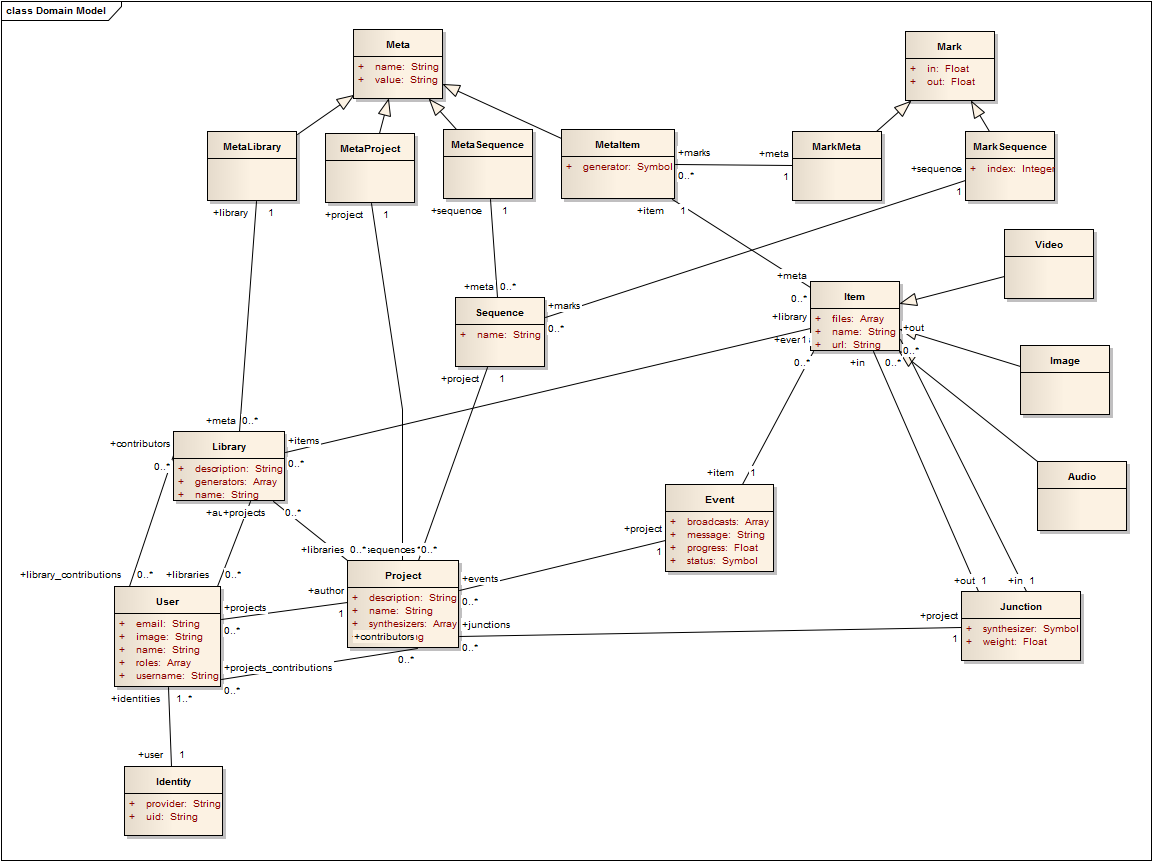
\includegraphics[width=1\textwidth]{./obrazova_priloha/domain_model.png}
\caption{Doménový model celého projektu Narra}
\end{figure}

\par User reprezentuje přihlášeného uživatele, který chce používat aplikaci. Každý uživatel může mít vazbu na projekt a knihovnu. Entita Item obsahuje informace o jménech souboru, url videa a vlastních stažených souborů. Dále obsahuje vazby na knihovnu, ve které je uložen sám Item. Itemy se podle definice v modelu nemohou vyskytovat samostatně, musí být organizovány v knihovnách. V případě mého projektu nebudu vytvářet Item ale jeho potomka Video. 
\par Další vazba je na entity MetaItem, které reprezentují generátor pro metadata. MetaItem je třídní potomek Meta, který přebírá atributy rodiče, jež jsou povinné. Při ukládání položek v Meta musí být vyplněno Meta.name i Meta.value. Po prozkoumání doménového modelu NARRA jsem vytvořil můj model viz obrázek 2.2.

\begin{figure}[H]
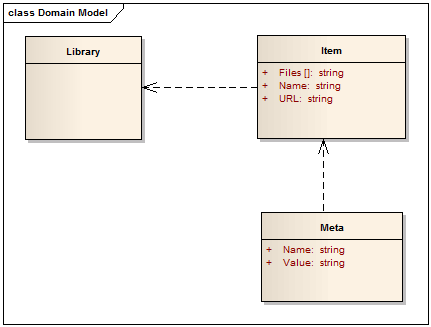
\includegraphics[width=1\textwidth]{./obrazova_priloha/domain_my.png}
\caption{Doménový model mé části Narry}
\end{figure}
\par Moje část aplikace se týká především entit Video, MetaItem a Library. Entita Library reprezentuje celou knihovnu videí, se kterou se bude lokálně pracovat. Video (potomek Item) je entita, které budu při vytváření asistovat poskytnutím URL při zadávání. Po zadání budu muset zpracovat obsah odkazu a vrátit metadata a cestu ke stažení videa. Jméno pro konkrétní prvek je reprezentováno řetězcem a url je také řetězec. Pro jednoduché volání budu mít vytvořenou třídu Connector, potomka Narra::SPI, která bude provádět inicializace, validaci, popis metadaty a stažení videa a případných titulků.
\par Zpracování videa probíhá vytvořením nového prvku (Item) v knihovně. Pro zpracování se použije POST požadavek s parametry v1/items/new (author, admin). Po zpracování dostaneme strukturu nově vytvořeného prvku (Item).
\par Příklad POST požadavku\cite{narra_en}:
\begin{verbatim} 
POST v1/items/new
url: "http://example.org/00329O-051.mov"
library: "552a328961633276b1000000" 
author: "Camera Guy"
metadata: {"description": "Some interesting description"}
\end{verbatim}
\hfill
\par Příklad odpovědi:
\begin{verbatim}
{"status":"OK","item":{
  "id":"552a338961633277b1000000",
  "name":"00329O-051",
  "url":"http://example.org/00329O-051.mov",
  "type":"video",
  "prepared":false,
  "library":{"id":"552a...b1000000","name":"Example Library"},
  "metadata":[
   {"name":"type","value":"video","generator":"source"},
   {"name":"name","value":"00329O-051","generator":"source"},
   {"name":"url","value":"url","generator":"source"},
   {"name":"library","value":"test","generator":"source"},
   {"name":"author","value":"testovaci","generator":"source"},
   {"name":"description","value":"test","generator":"bob"}
  ]
}}
\end{verbatim}
\par V odpovědi jsem musel zkrátit identifikátor knihovny, aby se mi vešel výraz na stránku. Ze stejného důvodu jsem byl nucen zkrátit hodnotu url. Zde je možné nastavit, zda bude projekt veřejný. V takovém případě je možné dostat přístup pouze pro čtení za předpokladu, že je knihovna součástí projektu. Pro vyšší práva je nutností být contributor (spolupracovník) daného projektu. Získání výpisu přístupných knihoven se provádí GET požadavkem na zdroj/adresu v1/libraries(author/admin).
\section {MongoDB}
\par MongoDB\cite{mongodb} je multiplatformní NoSQL databáze. Nepoužívá klasické tabulky, založené na relační struktuře, ale má svá vlastní schémata ve formáto BSON\cite{mongogbinc}. Objektová databáze umožňuje rychlejší a lehčí integraci dat. Tvůrcem NoSQL databáze je Americká společnost MongoDB\cite{mongodb} Inc. založená v roce 2007. V roce 2009 přešla společnost MongoDB\cite{mongodb} k open source řešení a stala se součástí významných společností, například BOSH.
\subsection {Formát BSON}
\par Formát BSON\cite{mongogbinc} je nejvíce využíván při ukládání a přenosu dat po síti v neobjektové databázi. Je velmi podobný již známému JSON formátu. Ukládání dat probíhá v binární formě, což je efektivnější z hlediska rychlosti i paměťové náročnosti. V některých případech bude BSON zabírat o něco více místa, neboť potřebuje hlavičku, ve které je uložena délka pole s daty.
Například formát JSON bude uložený v BSON\cite{mongogbinc}u takto: 

\begin{table}[h]
\caption[MongoDB příklad formátu BSON]{MongoDB příklad formátu BSON}\label{tab:bson}
\begin{tabulary}{\textwidth} {| l | l | l |}
 						& \textbackslash{x}16\textbackslash{x}00\textbackslash{x}00\textbackslash{x}00 								&// total document size \\
 						& \textbackslash{x}02 																						&// 0x02 = type String\\
\{"hello": "world"\} 	& hello\textbackslash{x}00 																					&// field name\\
 						& \textbackslash{x}06\textbackslash{x}00\textbackslash{x}00\textbackslash{x}00world\textbackslash{x}00 		&// field value\\
 						& \textbackslash{x}00 																						&// 0x00 = type EOO \\
\end{tabulary}
\end{table}
\vfill



                   
  
  

\section{YouTube API}
\subsection{Youtube API V3}
\section {Testovací nástroj RSpec}
\subsection{Historie}
\par RSpec\cite{davidchelimsky2015} je~samostatný testovací nástroj psaný v~Ruby, který vznikl jako experiment Stevena Bakera, Davida Astelse a~Aslaka Hellesøe. S vývojem začali v~roce 2006 na Ruby on~Rails, neboť okolo roku 2006 byly Ruby on~Rails nejpoužívanější Ruby aplikace. Pomocí RSpec lze testovat libovolný kód v~Ruby. První vydaná verze 1.0 vyšla o~rok později a~obsahovala funkce, které má RSpec dodnes. Měl ovšem několik ne úplně efektivně naimplementovaných částí a~proto musel být přepsán.
\par Koncem roku 2008 zabudoval Chad Humphries \uv{Micronauta}, který v~sobě obsahoval systém metadat a~poskytoval mnohem lepší flexibilitu než RSpec 1.0. V roce 2010 začali David a~Chad pracovat na verzi 2. Chtěli celý projekt rozdělit do modulů, které by pak mohli používat samostatně a~navazovat jedním na druhý. Jako jádro posloužil Micronaut, na který navazovali moduly.
\par Listopad roku 2012 byl pro vývor RSpecu zlomový. David Asteles se~rozhodl od projektu odpojit a~věnovat se~jiným věcem. Lídrem pro RSpec se~stal Myron Marston a~pro rspec-rails byl nominován Andy Linderman. Nově vytvořený tým začal pracovat na verzi RSpec 3, která byla spojením a~vyčištěním všech předchozích verzí dohromady. Po vydání RSpec 3 odešel Andy Linderman do důchodu. Dodnes se~RSpec rozvíjí díky velké komunitě spolupracovníků.
\par V mé Bakalářské práci budu pracovat s~jádrem testovacího nástroje RSpec a~očekáváními, neboli \texttt{expectations}. V následujících dvou podkapitolách uvedu postup instalace a~ukázky použití daných komponent.

\subsection{RSpec core}
\par RSpec core je~samotné jádro aplikace, na které navazují další moduly. Je nezbytnou částí pro testování. Instalace je~složená ze tří příkazů \textit{gem install rspec}; \textit{gem install rspec-core}; \textit{rspec --help} pro nápovědu k nově nainstalovanému softwaru. První příkaz nainstaluje rspec-core, rspec-expectations a~rspec-mocks, což je~kompletní balíček pro testování. Druhý příkaz nainstaluje pouze rspec-core, který neobsahuje všechny funkčnosti. 

\par Základní struktura popisu testů je~velmi podobná hovoru v~angličtině. Používají se~slova \uv{describe} a~\uv{it}, která mají stejný význam jako v~mluveném slově.

\par Dále můžeme deklarovat vnořené skupiny pomocí klíčových slov \texttt{describe}, nebo \texttt{context}. Tato klíčová slova nakonec zavolají příslušné metody, což je~pro programátora skryto jazykem DSL, kterým popis testů v~systému RSpec rozhodně je. Pro lepší představu, jak se~dá napsat test v~jazyce Ruby, zde uvádím jednoduchý příklad:
\begin{minted}{ruby}
RSpec.describe Order do
  context "with no items" do
    it "behaves one way" do
      # ...
    end
  end

  context "with one item" do
    it "behaves another way" do
      # ...
    end
  end
end
\end{minted}
Další ukázky z rspec-core podrobněji rozeberu v~části testování ke konci mé práce.

\subsection{RSpec expectations}
\par Instalace balíčku expectations je~naprosto stejná jako instalace rspec-core, ba i jednodušší. Stačí napsat pouze \textit{gem install rspec}, pro použití s~rspec core. V případě testování jinými nástroji, které podporují expectations, je~příkaz lehce odlišný \textit{gem install rspec-expectations}.

%Pro použití ve vývojářském režimu master \note{?} je~potřeba doplnit na začátek souboru \note{jakého:} tento kus kódu:
%\begin{minted}{ruby}
%%w[rspec-core rspec-expectations rspec-mocks rspec-support].each do |lib|
%  gem lib, :git => "git://github.com/rspec/#{lib}.git", :branch => 'master'
%end
%\end{minted}
%\note{Toto je~předpokládám výtažek z nějakého Gemfile, který ale funguje jen tehdy, pokud se~používá bundler. Respektive aby se~tyto gemy nainstalovaly, musí se~spustit \texttt{bundle install}, což ale nezaručuje dostupnost daných balíčků přes celý systém, ale jen pro tuto konkrétní aplikaci.}

\par Použití je~velmi intuitivní, neboť je~naprosto shodné s~projevem v~angličtině. Velmi hrubá forma je~expect(z čeho).operace(s čím). Souvislý kód poté vypadá například takto:
\begin{minted}{ruby}
RSpec.describe Order do
  it "sums the prices of the items in its line items" do
    order = Order.new
    order.add_entry(LineItem.new(:item => Item.new(
      :price => Money.new(1.11, :USD)
    )))
    order.add_entry(LineItem.new(:item => Item.new(
      :price => Money.new(2.22, :USD),
      :quantity => 2
    )))
    expect(order.total).to eq(Money.new(5.55, :USD))
  end
end
\end{minted}

\par Zde máme metodu Order, ve které vytvoříme dvě položky. První má hodnotu (1.1, :USD) a~druhá (2.2, USD), kterou jsme ovšem vytvořili pomocí \texttt{:quantity => 2} dvakrát. Proto můžeme otestovat, zda součet těchto tří prvků je~roven (5.5, :USD). Návratová hodnota testování pomocí expect je~true/false. V případě negativního / neočekávaného výsledku oznámí terminál, co očekával a~na dalším řádku co dostal od programu. Velmi snadno se~tedy pozná, kde nastala chyba. V tabulce 2.2\cite{rspectable} jsou uvedeny příklady testovacích příkazů.

\begin{center}
\begin{longtable}{| m{.38\textwidth} | m{.55\textwidth} |} 
\hline
 \textbf{Zabudované komparátory} & \textbf{Význam} \\ 
 \hline
 expect(actual).to eq(exp) & Rovná se~( == ) \\
 \hline
 expect(actual).to eql(exp) & Rovná se~( eql? ) \\
 \hline
 \multicolumn{2}{||c||}{\textbf{Identita}}\\
 \hline
 expect(actual).to be(exp) / to equal() & Zda je~identické\\
 \hline
 \multicolumn{2}{||c||}{\textbf{Porovnání}}\\
 \hline
 expect(actual).to be(exp) > / < / >= / <= expected & Operace porovnání \\
 \hline
 \multicolumn{2}{||c||}{\textbf{Regelární výrazy}}\\
 \hline
 expect(actual).to match(/exp/) & Zda výraz odpovídá exp \\
 \hline
 \multicolumn{2}{||c||}{\textbf{Třídy}}\\
 \hline
 expect(actual).to be\_an\_instance\_of(exp) & Jestli se~aktuální třída == exp \\
 \hline
 expect(actual).to be\_a(exp) & Alias k předchozímu \\
 \hline
 expect(actual).to be\_an(exp) & Alias k předchozímu  \\
 \hline
 expect(actual).to be\_a\_kind\_of(exp) & Alias k předchozímu  \\
 \hline
 \multicolumn{2}{||c||}{\textbf{Boolovské true / false}}\\
 \hline
 expect(actual).to be\_truthy  & Projde když actual != nil OR false\\
 \hline
 expect(actual).to be true    & Projde když actual == true \\
 \hline
 expect(actual).to be\_falsy   & Projde když actual == nil OR false \\
 \hline
 expect(actual).to be false   & Projde když actual == false \\
 \hline
 expect(actual).to be\_nil     & Projde když actual == nil \\
 \hline
 expect(actual).to\_not be\_nil & Projde když actual != nil \\
 \hline
 \multicolumn{2}{||c||}{\textbf{Očekávání errorů}}\\
 \hline
 expect \{ ... \}.to raise\_error & Očekávání, že ... vyvolá error \\
 \hline
 expect \{ ... \}.to raise\_error(ErrorClass) & Očekávání, že ... vyvolá error z ErrorClass\\
 \hline
 expect \{ ... \}.to raise\_error("message") & Očekávání, že ... error bude stejný jako "message" \\
 \hline
 expect \{ ... \}.to raise\_error(ErrorClass, "message")  & Kombinace druhé a~třetí varianty \\
 \hline
 \multicolumn{2}{||c||}{\textbf{Vyhození chyby}}\\
 \hline
 expect \{ ... \}.to throw\_symbol & Očekávání vyhození libovolného symbolu\\ 
 \hline
 expect \{ ... \}.to throw\_symbol(:symbol) & Očekávání vyhození symbolu :symbol\\ 
 \hline
 expect \{ ... \}.to throw\_symbol(:symbol, 'value') & Vyhození symbolu :symbol s~hodnotou 'value'\\ 
 \hline
 \multicolumn{2}{||c||}{\textbf{Členství v~kolekci}}\\
 \hline
 expect(actual).to include(expected) & Splněno, když actual obsahuje expected \\
 \hline
 expect(actual).to start\_with(expected) & Actual začíná expected \\
 \hline
 expect(actual).to end\_with(expected) & Actual končí expected \\
 \hline
 \caption[RSpec metody testování]{Různé způsoby testů pomocí RSpec}\label{tab:rspec}
\end{longtable}
\end{center}

\section{Ruby balíčky(gems)}
\par RubyGems\cite{elmendorfdirk2006} je~obdoba linuxového manageru balíčků pro programovací jazyk Ruby. Umožňuje snadné stažení a instalaci balíčků do systému. Stejně jako linuxové balíčky hlídá i tento balíčkovací systém závislosti, verze. Na adrese \url{https://rubygems.org/} se~dají nainstalovat publikované balíčky, popřípadě pomocí aplikace bundler lze získat i nepublikovaný software z repozitáře na GitHubu. 
\section{Vyrovnávací paměť médií}
\subsection{Obecný popis}
\par 
\subsection{Realizace v projektu NARRA}
\par // todo


1) Tvůj konektor poskytne informaci kde se nachází soubor s multimediálním obsahem.
2) Pracovní server NARRA navštíví tuto adresu (kterou hostuji na tom download serveru), čímž dojde ke stažení videa, uložení na cestu dotupnou přes http a zaslání hlavičky 303 s lokací souboru.
3) Pracovní server tedy náseduje přesměrování. (k timeoutu nedochází)
4) Pracovní server přepočítá videosoubor do všech formátů potřebných v NARRA (WebM ve vysoké a nízké kvalitě; zvukový soubor ve formátu OGG Vorbis) odkazy na tyto soubory sám předá do databáze NARRA
\section {Kodek VP8 a ukládání videí v~NARRA}
\par Pro správné pochopení významu kodeku VP8\cite{vp8} je potřeba trocha teorie k WebM\cite{webm}. WebM je otevřený formát multimediálních souborů používaný na webu. WebM soubory se skládají z obrazových toků komprimovaných právě kodekem VP8, nebo VP9. V projektu NARRA je použita komprimace pomocí VP8. V aktuálním nastavení se videa počítají do formátu WebM (video v~kodeku VP8, audio ve Vorbis) ve dvou kvalitách: 720p s bitrate 1Mbps a 180p s bitrate 300kbps. Navíc je počítán čistě zvukový náhled ve Vorbis (kontejner OGG) a pět náhledů v~rozlišení 350x250 ve formátu PNG. 
\par Pro uložení videa se používá kontejner (například WebM, MP4, AVI, MOV, \ldots), tyto formáty definují vnitřní strukturu a složení jednotlivých datových proudů do výsledného souboru. Tento datový proud je potřeba zkomprimovat. K účelu komprimace slouží právě kodek (MPEG, VP8, H.264, \ldots). Komprimace slouží pro zmenšení datového toku pro záznam videa.
\subsection{VP8}
\par Jak již bylo zmíněno VP8 je formát pro kompresi dat vlastněný společností Google. Je založen na knihovně \texttt{libvpx}, která jediná umí zakódovat VP8 video stream. Dekódování probíhá také pomocí Google knihovny \texttt{libvpx}.
\chapter{Realizace}
\section{Řešení spolupráce s~YouTube API}
\subsection{YouTube Data API (v3)}
\par API v3 umožňuje začlenění funkcí YouTube do vlastní aplikace. Proto jí používám pro získání metadat. Nejprve jsem si musel vytvořit google účet a~zaregistrovat aplikaci. Pro vytvoření google účtu a~zaregistrování slouží \url{https://console.developers.google.com/project}. Každý takto vytvořený projekt má u sebe statistiky s~počtem dotazů, počtem chyb, identifikačním řetězcem a~názvem. 
\par Po kliknutí na název mého projektu je možné se dozvědět podrobnější informace a~změnit konfiguraci projektu. Základní náhled mi poskytuje graf s~počtem požadavků, kde vidím jak moc vytěžuji YouTube API. Dále je zde potřeba nechat si vygenerovat unikátní API klíč, pomocí kterého získávám metadata.

\section{Třída connector}
\subsection{Založení aplikace}
\par Před založením aplikace jsem několikrát navštívil R.U.R. v Praze, kde se projekt NARRA vyvýjí a po vymyšlení mé části aplikace jsem požádal vedoucího práce, aby mi daný projekt předpřipravil, neboť na fork projektu z NARRA jsem neměl dostatečná práva. Pro lehčí kontrolu mého postupu a možnost verzování jsem zvolil \url{www.github.com}. Po předpřipravení projektu podle mého návrhu jsem si na githubu vytvořil účet, vlastní SSH klíč a mohl jsem si celou aplikaci k sobě natáhnout a začít programovat.

\subsection{Validace a inicializace}
\par Vlastní implementace je napsaná v jazyce Ruby a~vývojovém prostředí RubyMine. Pro vyřešení metadat jsem si vytvořil jednu třídu, kterou jsem napojil na narra-core. Dále jsem potřeboval knihovny net/http a json pro snažší práci.
\begin{minted}{ruby}
require 'narra/core'
require 'net/http'
require 'json'

module Narra
  module Youtube
    class Connector < Narra::SPI::Connector
\end{minted}
\par Tímto kusem kódu jsem vytvořil nový modul, který je potomkem Narra::\-SPI::Connector. Další věc jsem musel řešit validaci url. V případě nevalidní url mi stačilo vrátit false, při úspěchu jsem vracel true. Nejdřívě jsem zkoušel do projektu zakomponovat metodu match. Ta ovšem vracela string místo booleovké hodnoty a~proto jsem ji musel nahradit =\~. Takto zkonstruovaný výraz by ovšem nefungoval úplně dokonale, neboť při funkční url by vrátil 0. Stačilo výraz lehce poupravit do tvaru !!(url =\~ RegExp ) a~vše fungovalo jak má.
\begin{minted}{ruby}
!!(url =~ /^(?:http:\/\/|https:\/\/)?(www\.)?(youtu\.be\/|youtube
\.com\/(?:embed\/|v\/|watch\?v=|watch\?.+&v=))((\w|-){6,11})(\S*)
?$/
\end{minted}

\par Regulární výraz je matematický formalismus pro popis slov/vět jazyků. Jedná se tedy o způsob jak formálně popsat určité slovo, případně větu pomocí formálního vyjádření speciálními symboly a skupinami znaků. V ruby je popis regulárním výrazem uvozen / na začátku a / na konci. Pomocí dvou lomítek řekneme překladači, že zápis uvnitř lomítek má považovat za regulární výraz.
\par V předchozím regulárním výrazu jsem použil standartní konstrukce, až na jednu vyjímku, která není až tak obvyklá. Jedná se o ?:výraz, což znamená že bude splněno při žádném nebo jednom výskytu výrazu. Všechny ostatní konstrukce jsou popsány v následující tabulce. Ruby má také velmi dobrou webovou podporu pro testování regulárního výrazu na stránkách \url{http://rubular.com/}.

\begin{table}[h!]
\centering
\caption[Tabulka skupin symbolů pro regulární výraz]{Tabulka skupin symbolů pro regulární výraz}\label{tab:regexpr}
\begin{tabular}{| p{.20\textwidth} | p{.80\textwidth} |}
\hline
\verb|[abc]| & Právě jeden znak z množiny: a, b, c. \\
\hline
\verb|[^abc]| & Právě jeden znak z doplňku množiny: a, b, c. \\
\hline
\verb|[a-z]| & Právě jeden znak z rozsahu a-z. \\
\hline
\verb|[a-zA-Z]| & Právě jeden znak z rozsahu a-z nebo A-Z. \\
\hline
\verb|^| & Znak pro začátek řádky. \\
\hline
\verb|$| & Znak pro konec řádky, např \verb|[a-z]+$| bude uspokojen všemi řetězci tvořenými znaky a-z, který se vyskytne alespoň jednou a bude před koncem řádky. \\
\hline
\verb|\A| & Začátek řetězce. \\
\hline
\verb|\z| & Konec řetězce. \\
\hline
\verb|.| & Jakýkoli znak. \\
\hline
\verb|\s| & Jakýkoli znak tvořený bílími znaky. \\
\hline
\verb|\S| & Jakýkoli znak netvořený bílími znaky. \\
\hline
\verb|\d| & Číslice. \\
\hline
\verb|\D| & Vše krom číslice. \\
\hline
\verb|\w| & Jakýkoli znak z množiny (písmeno, číslo, podtržítko). \\
\hline
\verb|\W| & Opak \verb|\w|. \\
\hline
\verb|\b| & Shoda musí nastat na hranici číselného a nečíselného znaku. \\
\hline
\verb|(...)| & Musí se shodovat přesně s výrazem v (), např (http)* značí nula až nekonečno opakování http. \\
\hline
\verb|(a|b)| & Znak a nebo b, a i b mohou být i skupina znaků. \\
\hline
\verb|a?| & Žádný, nebo právě jeden výskyt a. \\
\hline
\verb|a*| & Žádný, nebo více výskytů znaku a. \\
\hline
\verb|a+| & Jeden, nebo více výskytů znaku a. \\
\hline
\verb|a{3}| & Přesně tři výskyty znaku a. \\
\hline
\verb|a{6,}| & Šest a více výskytů znaku a. \\
\hline
\verb|a{3,6}| & Mezi třemi a šesti výskyty znaků a. \\
\hline
\end{tabular}
\end{table}

\par Pro správnou funkčnost ověření, zda je url validní či ne, bylo potřeba vyřešit přesměrování. Například url adresa, která nevypadá ani z části jako validní může vést k youtube videu. Příkladem takové adresy je \url{http://goo.gl/TKMZjS}. Pouhým ověřením přes regulární výraz bych neměl šanci zjistit obsah a validitu odkazu. 

\subsection{Přesměrování}
\par Přesměrování vyžadovalo novou knihovnu net/http, ze které jsem použil její zabudované metody. Při vytváření jsem nastavil horní hranici přesměrování na 20, neboť drtivá většina proběhne do tří požadavků. Dále jsem potřeboval zajistit, abych se netočil dokola na několika málo url, což by bylo neefektivní a hloupé. Pro maximum dvaceti prvků mi bohatě postačuje pole s lineárním procházením, neboť hash mapa by byla zbytečný luxus. Takto se mohu podívat zda jsem již nenavštívil nějakou url dvakrát, což by znamenalo zacyklené přesměrování a v mém případě vyhození příslušné vyjímky.
\par První úskalí knihovny net/http nastalo v okamžiku, kdy url neměla v názvu protokol. V tomto případě nebyla schopna rozpoznat server a celý proces zkolaboval. Řešením bylo přidat k url bez protokolu protokol http, který se v případě potřeby přesměruje na https. Kdybych přidal místo pouhého http rovnou https, mohlo by se stát, že některé stránky nebudou fungovat, neboť není zaručené zpětné přesměrování z šifrovaného protokolu na nešifrovaný.
\par Poslední část přesměrování spočívala ve zjištění příslušného kódu, kterým mi stránka odpověděla na get pořadavek. Při kódu 2xx je vše v pořádku a url lze rovnou vrátit, neboť každý jistě ví, že 2xx kód je symbolem úspěchu. Číslovka začínající trojkou je ovšem zajímavějším protože se jedná o přesměrování. V tomto případě musí programátor zjistit, na kterou stránku se dostane a proces opakovat, než dostane kód 2xx, nebo než zjistí, že je v cyklu. Poslední skupina jsou kódy 4xx a 5xx značící chybu klienta a chybu serveru.

\par Po zjištění, zda je požadovaná url adresa validní, bylo potřeba ještě provést inicializaci. Zde vytáhnu z YouTube API všechny potřebné informace o videu, které budu dále zpracovávat. Zde je velké množství parametrů, které YouTube API nabízí k výběru. Dále je potřeba vygenerovaný API klíč, pomocí něhož YouTube pozná, komu ubrat denní kvótu za požadavek. V následující tabulce je příklad parametrů pro API.

\begin{table}[h!]
\centering
\caption[Parametry YouTube API a jejich význam]{Parametry YouTube API a jejich význam}\label{tab:apiparams}
\begin{tabular}{| l | l |}
\hline
Parametr & Význam \\
\hline
snippet & Zobrazí hlavní informace o videu \\
\hline
contentDetails & Zobrazí detaily obsahu \\
\hline
fileDetails & Zobrazí detaily souboru \\
\hline
player & Zobrazí detaily přehrávače \\
\hline
processingDetails & Zobrazí podrobnosti zpracování \\
\hline
recordingDetails & Zobrazí podrobnosti nahrávání \\
\hline
statistics & Zobrazí statistiky videa \\
\hline
status & Zobrazí status \\
\hline
suggestions & Zobrazí návrhy \\
\hline
topicDetails & Zobrazí detaily o tématu videa \\
\hline
\end{tabular}
\end{table}

\par Konrétní požavavek byl na adresu \url{https://www.googleapis.com/youtube/v3/videos?id=#{@videoid}&key=klíč&part=část}, kde @videoid je inicializovaná hodnota pro identifikátor videa, klíč je unikátní API klíč programátora a část je jeden, nebo několik parametrů oddělených čárkou. Zde je nutné vzít v potaz, že za vytížení YouTube serveru se platí a v jistých případech nemalou částí denní přidělené kvóty jednotek. Detailní výpočet jsem popsal již v kapitole o YouTube API, zde se o tomto omezení zmiňuji podruhé, neboť jsem nepoužil všech deset parametrů, ale jen čtyři.
\par Snippet, který napíše o videu většinu informací. ContentDetails byl potřeba pro splnění pořadavků z DublinCore, statistics přidají do obsahu počty sledovaností a~status zobrazí licenci a~informace o sdílení videa. Tyto čtyři položky stačí pro pořadovaná metadata zadavatelem a~při přidání dalších bych zbytečně omezoval maximální počet vrácených položek díky omezení YouTube API a aplikace by pozbývala na efektivitě.
\par Při inicializaci je druhý parametr klíč, který slouží 


\par Nyní již mám k dispozici json objekt a můžu se pustit do práce. První pokus o rozparsování proběhl ručně. Vždy jsem si pomocí methody split rozdělil objekt na pole o dvou částech a druhý index jsem rozdělil znovu podle čárky a odřádkování. Pro lepší představu o vizuální stránce kódu sem dám ukázku vytažení obsahu title.
\begin{minted}{ruby}
pom = @youtube_json_object_snippet.split('"title": "')[1]
@name = pom.split("\",\n")[0]
\end{minted}
\par Toto řešení bylo vcelku jednoduché, rozdělení podle ",\verb|\|n bylo v pořádku, neboť YouTube v popiscích provedlo escapacování těchto znaků a nemohlo dojít k nechtěnnému rozdělení ve špatném místě. Kód ovšem vypadal naprosto hrozně a proto jsem zvolil již hotovou variantu json parseru. Pro porovnání ukázka kódu s knihovnou json.
\begin{minted}{ruby}
my_hash = JSON.parse(@youtube)
my_hash["items"][0]["snippet"]["title"]
\end{minted}

\par Toto řešení je mnohem přehlednější a další programátor má usnadněné pochopení vnitřní struktury json objektu. Po této odbočce se dostáváme zpátky k řešení, kde druhým zmiňovaným způsobem vracím název videa samostatně a ne v komplexní struktuře metadat. Tato alternativa byla zvolena záměrně díky ukládání videí v mateřském projektu. Dalším požadavkem mateřkého projektu bylo vrácení typu videa :video. Tím jsem měl za sebou základní část a mohl jsem pokračovat s metadaty.


\subsection{Metadata}

\par Pro popis metadaty jsem vycházel ze struktury DublinCore, která ovšem ne úplně 100\% odpovídala mé představě a představě youtube vývojářů a proto jsem celou kostru musel upravit. 

\begin{table}[!ht]
\centering
\caption[Metadata předávaná do NARRA]{Metadata předávaná do NARRA}\label{tab:bson}
\begin{tabular}{| p{.30\textwidth} | p{.70\textwidth} |}
\hline
	Název & Obsah \\
\hline
\hline
	videoId & Jednoznačný identifikátor videa. \\
\hline
	channelId & Jednoznačný identifikátor kanálu, pod kterým je video k dispozici. \\
\hline
	channelTitle & Název kanálu, pod kterým je video k dispozici. \\
\hline
	publishedAt & Přesný čas vydání a zvěřejnění videa. \\
\hline
	description & Popis k videu. \\
\hline
	categoryId & Číslo kategorie, do které patří dané video. \\
\hline
	liveBroadcastContent & Booleovská hodnota, zda je obsah ve videu vysílaný živě. \\
\hline
	viewCount & Počet shlédnutí videa. \\
\hline
	likeCount & Počet udělení líbí se. \\
\hline
	dislikeCount & Počet udělení nelíbí se. \\
\hline
	favouriteCount & Počet přidání do oblíbených. \\
\hline
	commentCount & Počet komentářů k videu. \\
\hline
	duration & Čas trvání. \\
\hline
	dimension & Zda je video 2d, nebo 3d. \\
\hline
	definition & Jaké je maximální možné rozlišení videa. \\
\hline
	caption & Booleovská hodnota, zda video obsahuje či neobsahuje titulky. \\
\hline
	licensedContent & Zda obsah videa podléhá licencování. \\
\hline
	regionRestriction & Zda je video zakázané v nějaká zemi. \\
\hline
	uploadStatus & Zda je nahrané video již kompletní, či ještě ne. \\
\hline
	privacyStatus & Informace o soukromí videa. \\
\hline
	license & Kdo vlastní licenci k videu. \\
\hline
	embeddable & Zda je možné toto video použít k vložení. \\
\hline
	publicStatsViewable & Booleovská hodnota o zobrazitelnosti veřejných statistik. \\
\hline
	timestamp & Čas ve formátu utc, kdy byla metadata pořízena. \\
\hline
\end{tabular}
\end{table}

\par Jak jste si mohli povšimnout v této tabulce mi chybí titulek videa. Toto řešení je součástí návrhu, kde vracím název videa samostatně pro lepší následné ukládání v mateřském projektu. Dále mám staticky zadefinovaný typ videa, který se nemění. 
\par Pro správné pochopení, jak extrhahovat metadata ze struktury JSON objektu je potřeba zjistit jak přesně vypadá. Celý objekt je jeden prvek obsahující pole items, ze kterého používám nultý prvek. V této úrovni rozhoduji, zda vyberu data z položky snippet, statistics, contentDetails nebo status. Po zvolení například snippet se dostanu o úroveň hlouběji a mohu vybrat konkrétní položku, například channelId. Stejným způsoben jsou dostupná všechna metadata z JSON objektu, pouze u restrikce zemí vzacím složitější strukturu než string.
\par Poslední prvek metadat timestamp nenajdu v DublinCore ani v YouTube API, je ovšem důležité ho do dat zařadit, kvůli udržovatelnosti. V mateřské aplikaci bude nejspíš také časový otisk, který není v této chvíli ještě dodělán a proto jsem ho umístil do metadat. Je zde kvůli kontrole, jak staré jsou statistiky u videa a například pro automatizovanou kontrolu metadat starších než dva týdny se tento údaj hodí. Ještě jsem přemýšlel zda bude dobré řešení vložit časový otisk přímo do metadat, nebo raději mimo, ale řešení s otiskem v metadatech vyhrálo. Nejpádnější důvod byl, že při aktualizaci se zavolá pouze metoda metadata a nebude se muset volat žádná další, neboť znovu stahovat video nemá cenu, v případě přidání titulků se zavolá ještě download\_subtitles. Také jméno, identifikátor, url a typ videa se nebudou měnit.
\par Celkem můj gem poskytuje k jednomu videu 24 metadat a odděleně také jméno videa, typ videa. V součtu se jedná o dvacet šest položek, které umožní rychlejší vyhledávání a relevantní obsah pro každého uživatele, který moje rozšíření využije.

\subsection{Dokončení}
\par Na závěr mi zbývalo vrátit youtube url ve formátu, kde bude pouze video stream bez ostatních elementů, neboť ze standartní url by to bylo moc práce navíc pro jádro aplikace. Pro tento účel souží adresa \url{https://www.youtube.com/v/}, za kterou stačí přiřadit identifikátor videa a požadovaný video stream je na světe. 
\par Poslední kus kódu patřil stažení titulek. Na první pohled se to zdálo jako velmi jednoduchý úkol, ovšem stažení titulek stojí 200 jednotek. Proto je potřeba autentizace API klíčem. Tímto klíčem je potřeba být přihlášen již v jádru aplikace při spuštění a na můj konektor se jen dotázat na stažení titulek. Jelikož je ještě autentizace pomocí OAuth v mateřském projektu nedořešená, předpřipravil jsem můj kus pro stažení titulek pouze pro aktuální funkčnost, která zabezpečí, že po autentizaci pomocí OAuth začne mé stažení titulek fungovat.
\par Titulky k videu jsou k dispozici z \url{https://www.googleapis.com/youtube/v3/captions/}, za kterou se opět přiřadí identifikátor videa. Bez autorizace ovšem nahlásí stránka chybový kód: "Login Required".

\section{Testování YouTube konektoru}
\subsection{Teorie testování}
\par Pro správné pochopení teorie testování\cite{si1} si musíme uvědomit, že pomocí testů prokážeme že software obsahuje chyby při nesplnění testu. Při splnění všech testů nemůžeme dokázat, že je software stoprocentně bez chyb, neboť může existovat chyba, kterou testy neodhalily. Proto je potřeba se důkladně věnovat testování, abychom snížili riziko chyby na nejnižší možnou úroveň.
\subsection{Jednotkové testy}
\par První druh testů jsou jednotkové testy\cite{si1}. Ty se zabývají konkrétní funkčností jednotlivých metod a~tříd. Testování probíhá pro jednu konkrétní třídu, obvykle běží krátkou dobu a~testování probíhá na lokálním počítači vývojáře. Tyto testy pokrývá v Ruby nástroj RSpec, který jsem popsal na začátku práce. V mých testech jsem se zaměřil na zjištění správné odezvy metod a~získání správných výsledků.
\subsection{Integrační testy}
\par Integrační testování\cite{si1} se provádí po dokončení jednotkových testů a~slouží k bezchybnému začlenění nového kusu aplikace do stávajícího projektu. Těmito testy se ověřuje nejen integrace komponentů, ale i spolupráce se softwarem případně hardwarem při složitějších projektech, které potřebují specifický hardware nebo software. 
\par Testování probíhá začleněním jedné z komponent a~postupném přidávání dalších komponent k celému projektu. Integrační testování je často zanedbáváno díky rozpočtu projektu. Takto nezachycené chyby se ovšem projeví v dalších testech a~je proto dobré integrační testy nepřeskočit.
\subsection{Systémové testy}
\par V pořadí již třetí zkouška funkčnosti projektu se zabývá chováním celého projektu jako celku. Provádí se zde simulace scénářů a~kroků, které mohou po nasazení projektu nastat. Je to poslední testování před předáním projektu zákazníkovi a~proto obvykle probíhá několikrát. Systémové testování\cite{si1} je nezbytné pro výstupní kontrolu projektu.
\subsection{Akceptační testy}
\par Akceptační testy jsou prováděné zákazníkem spolu se zástupcem firmy na předem dohodnutých scénářích. Jedná se o otestování, zda zadavatel správně pochopil požadavky zákazníka. Odhalení závažných nedostatků v této poslední fázi bývá nejhorším možným scénářem pro vývojáře, který musí následně aplikaci předělávat. Můj gem jsem testoval jednotkovými a~integračními testy, neboť systémové a~akceptační testování zajišťují programátoři jádra projektu.


\subsection{Testování třídy Connector}
\subsubsection{Testování URL}
\par První část testu kontroluje vytváření a~validaci URL. Před první částí testů jsem si nastavil testovanou URL a~zjistil, zda se správně vytvoří objekt dané třídy. Poté jsem zkontroloval tři globální proměnné, zda se nezměnil jejich obsah. Tyto dva testy zajistili primární funkčnost konektoru a~mohl jsem zkontrolovat konkrétní URL. Zde jsem hledal různé URL adresy, které nikam nepřesměrují a~jsou validní. Dále jsem potřeboval najít nevalidní URL, přičemž stačilo vhodným způsobem modifikovat URL validní. 
\par Poté jsem potřeboval najít URL, která se přesměruje na validní. Zde jsem použil funkci YouTube, kde je možné zvolit sdílení videa, což vytvoří zkrácenou URL, která se přesměruje. Poté jsem ještě použil Google zkracovač, což je také velmi dobrá metoda pro ověření validace a~přesměrování.
\subsubsection{Testování objektu konektoru}
\par Další testy již probíhaly pro určitý objekt konektoru. Zde jsem opět našel několik YouTube videí na kterých jsem testoval příslušná metadata. Pro hezčí zápis testu jsem chtěl zápis metadat převést z formátu \textit{\{name:'channelId', value:'\#\{@channelId\}'\}} do formátu \textit{\{'channelId'=>'\#\{@channelId\}'\}}, což mi umožnilo lepší a~přehlednější přístup k testování metadat. Url adresy jsem volil pro pokrytí speciálních znaků v popiscích, pro neobvyklá metadata, které jsou u videí jen zřídka a~pro pokrytí všech metadat. 
\par Zde byl problém s~proměnlivými statistikami u videa, kde například u počtu shlédnutí jsem musel při testování stále upravovat testovanou hodnotu. Proto jsem vizuálně otestoval s~JSON objektem shodu v proměnlivých počtech u statistik a~poté jsem test zakomentoval. Tento problém bych mohl vyřešit nastavením intervalu, což také není úplně nejlepší neboť bych se musel znovu podívat zda je to číslo opravdu dobře nebo ne.
\par V nástroji RSpec je v bloku \texttt{before} několik možností parametrů v závorkách. V první části testování, kdy jsem měl ještě málo testů, trval celý blok okolo deseti vteřin. V závěrečné fázi práce, kdy jsem otestoval vše co mě napadlo trval test i přes jednu minutu. Takto dlouhé testování se mi nezdálo a~proto jsem se důkladně zaměřil na parametrizaci v bloku \texttt{before}. Při parametru \texttt{:each}, který jsem měl ze začátku se celá inicializace provedla před každým blokem it, proto testy trvaly tak dlouhou dobu. Po změně na \texttt{:all} se rázem čas testů dostal stabilně pod deset vteřin. Proto je potřeba dávat velký pozor, zda neděláme v testu stejné věci zbytečně vícekrát.
\subsubsection{Testy na videích}
\par Pro první testované video jsem zvolil \uv{Zimní montáže - 1. díl} z kanálu mrk.cz. Zde byl zajímavý prvek ve formě odřádkování v popisu videa. Druhé testované video bylo znovu v duchu rybolovu s~zajímavým popiskem, který byl tentokrát prázdný. Dále jsem chtěl na druhém videu otestovat živé vysílání neboť toto video bylo vysíláno živě a~přesto je parametr \texttt{liveBroadcastContent} roven hodnotě \texttt{false}. Hodnota false byla v metadatech o videu správně, neboť po živém odvysílání video změní svůj stav a~není vysíláno živě.
\par Dále jsem vytvořil jeden test pro otestování titulků. Zde jsem potřeboval ověřit, zda mi program správě vyhodí výjimku při neexistujících titulcích. Tato výjimka je velmi opodstatněná, neboť každý download titulků stojí 200 jednotek z YouTube API kvóty a~bylo by nežádoucí nechat uživatele několikrát zkusit stáhnout neexistující titulky. Další test spočíval ve správném zpracování dlouhé URL adresy, obsahující další informace za identifikátorem videa, pomocí regulárního výrazu při validaci URL a~pro zkoušku vytažení všech dostupných dat.
\par Páté testované video bylo vytvořeno kvůli možnosti stáhnout validní titulky k videu. Další test vyzkoušel časovou známku u titulků pro čas vytvoření. Blok \uv{should check download video} měl na starost otestování možnosti stáhnout video, neboli dostat se na URL, která obsahuje pouze video stream. Tento test jsem nemohl provést, neboť potřebuji proměnnou prostředí, kterou dostanu až při dotazu na server. Předposlední test znovu zkusil stažení titulků a~ověření, zda bude vyhozena výjimka u neexistujících titulků.
\par Závěrečný test je zde z důvodu omezení videí v různých zemích. Zde YouTube předává hodnotu \texttt{blockedIn} v případě, že je video zakázáno v nějaké zemi. Seznam zemí dále vrátí pomocí pole. V případě, že video není nikde blokováno tento atribut zmizí, protože v databázi nemohou být prázdné hodnoty. Znovu jsem proto musel otestovat správné reagování na omezení.
\subsubsection{Shrnutí jednotkových testů}
\par V jednotkových testech jsem se snažil pokrýt všechny možné nástrahy, které mi je schopen uživatel nadělit a~otestovat, zda můj program reaguje podle předpokladů. Všechny testy proběhly bez chyb a~proto jsem snížil pravděpodobnost, že moje rozšíření obsahuje chyby na přijatelnou úroveň. S otestovaným softwarem pomocí jednotkových testů mohu pokračovat v integračních a~systémových testech s~mateřskou aplikací.
\subsection{Integrační testy}
\par Integrační testování odhalilo několik ošetření, které je potřeba provádět v mém balíčku a~nespoléhat na jádro aplikace. Jednalo se o zařazení metadat, která by měla hodnotu nil, nebo prázdný řetězec. V takovém případě jsem nesměl přidat danou položku s~metadaty k výslednému videu, neboť ošetřování obsahu metadat při zpracovávání videa by bylo v rozporu s~modelem. Další chybu integrační testy neodhalily a~má část aplikace funguje dle očekávání.
\begin{conclusion}
	%sem napište závěr Vaší práce
\end{conclusion}

\bibliographystyle{csn690}
\bibliography{mybibliographyfile}

\appendix

\chapter{Seznam použitých zkratek}
% \printglossaries
\begin{description}
	\item[GUI] Graphical user interface
	\item[XML] Extensible markup language
\end{description}


% % % % % % % % % % % % % % % % % % % % % % % % % % % % 
% % Tuto kapitolu z výsledné práce ODSTRAŇTE.
% % % % % % % % % % % % % % % % % % % % % % % % % % % % 
% 
% \chapter{Návod k~použití této šablony}
% 
% Tento dokument slouží jako základ pro napsání závěrečné práce na Fakultě informačních technologií ČVUT v~Praze.
% 
% \section{Výběr základu}
% 
% Vyberte si šablonu podle druhu práce (bakalářská, diplomová), jazyka (čeština, angličtina) a kódování (ASCII, \mbox{UTF-8}, \mbox{ISO-8859-2} neboli latin2 a nebo \mbox{Windows-1250}). 
% 
% V~české variantě naleznete šablony v~souborech pojmenovaných ve formátu práce\_kódování.tex. Typ může být:
% \begin{description}
% 	\item[BP] bakalářská práce,
% 	\item[DP] diplomová (magisterská) práce.
% \end{description}
% Kódování, ve kterém chcete psát, může být:
% \begin{description}
% 	\item[UTF-8] kódování Unicode,
% 	\item[ISO-8859-2] latin2,
% 	\item[Windows-1250] znaková sada 1250 Windows.
% \end{description}
% V~případě nejistoty ohledně kódování doporučujeme následující postup:
% \begin{enumerate}
% 	\item Otevřete šablony pro kódování UTF-8 v~editoru prostého textu, který chcete pro psaní práce použít -- pokud můžete texty s~diakritikou normálně přečíst, použijte tuto šablonu.
% 	\item V~opačném případě postupujte dále podle toho, jaký operační systém používáte:
% 	\begin{itemize}
% 		\item v~případě Windows použijte šablonu pro kódování \mbox{Windows-1250},
% 		\item jinak zkuste použít šablonu pro kódování \mbox{ISO-8859-2}.
% 	\end{itemize}
% \end{enumerate}
% 
% 
% V~anglické variantě jsou šablony pojmenované podle typu práce, možnosti jsou:
% \begin{description}
% 	\item[bachelors] bakalářská práce,
% 	\item[masters] diplomová (magisterská) práce.
% \end{description}
% 
% \section{Použití šablony}
% 
% Šablona je určena pro zpracování systémem \LaTeXe{}. Text je možné psát v~textovém editoru jako prostý text, lze však také využít specializovaný editor pro \LaTeX{}, např. Kile.
% 
% Pro získání tisknutelného výstupu z~takto vytvořeného souboru použijte příkaz \verb|pdflatex|, kterému předáte cestu k~souboru jako parametr. Vhodný editor pro \LaTeX{} toto udělá za Vás. \verb|pdfcslatex| ani \verb|cslatex| \emph{nebudou} s~těmito šablonami fungovat.
% 
% Více informací o~použití systému \LaTeX{} najdete např. v~\cite{wikilatex}.
% 
% \subsection{Typografie}
% 
% Při psaní dodržujte typografické konvence zvoleného jazyka. České \uv{uvozovky} zapisujte použitím příkazu \verb|\uv|, kterému v~parametru předáte text, jenž má být v~uvozovkách. Anglické otevírací uvozovky se v~\LaTeX{}u zadávají jako dva zpětné apostrofy, uzavírací uvozovky jako dva apostrofy. Často chybně uváděný symbol "{} (palce) nemá s~uvozovkami nic společného.
% 
% Dále je třeba zabránit zalomení řádky mezi některými slovy, v~češtině např. za jednopísmennými předložkami a spojkami (vyjma \uv{a}). To docílíte vložením pružné nezalomitelné mezery -- znakem \texttt{\textasciitilde}. V~tomto případě to není třeba dělat ručně, lze použít program \verb|vlna|.
% 
% Více o~typografii viz \cite{kobltypo}.
% 
% \subsection{Obrázky}
% 
% Pro umožnění vkládání obrázků je vhodné použít balíček \verb|graphicx|, samotné vložení se provede příkazem \verb|\includegraphics|. Takto je možné vkládat obrázky ve formátu PDF, PNG a JPEG jestliže používáte pdf\LaTeX{} nebo ve formátu EPS jestliže používáte \LaTeX{}. Doporučujeme preferovat vektorové obrázky před rastrovými (vyjma fotografií).
% 
% \subsubsection{Získání vhodného formátu}
% 
% Pro získání vektorových formátů PDF nebo EPS z~jiných lze použít některý z~vektorových grafických editorů. Pro převod rastrového obrázku na vektorový lze použít rasterizaci, kterou mnohé editory zvládají (např. Inkscape). Pro konverze lze použít též nástroje pro dávkové zpracování běžně dodávané s~\LaTeX{}em, např. \verb|epstopdf|.
% 
% \subsubsection{Plovoucí prostředí}
% 
% Příkazem \verb|\includegraphics| lze obrázky vkládat přímo, doporučujeme však použít plovoucí prostředí, konkrétně \verb|figure|. Například obrázek \ref{fig:float} byl vložen tímto způsobem. Vůbec přitom nevadí, když je obrázek umístěn jinde, než bylo původně zamýšleno -- je tomu tak hlavně kvůli dodržení typografických konvencí. Namísto vynucování konkrétní pozice obrázku doporučujeme používat odkazování z~textu (dvojice příkazů \verb|\label| a \verb|\ref|).
% 
% \begin{figure}\centering
% 	\includegraphics[width=0.5\textwidth, angle=30]{cvut-logo-bw}
% 	\caption[Příklad obrázku]{Ukázkový obrázek v~plovoucím prostředí}\label{fig:float}
% \end{figure}
% 
% \subsubsection{Verze obrázků}
% 
% % Gnuplot BW i barevně
% Může se hodit mít více verzí stejného obrázku, např. pro barevný či černobílý tisk a nebo pro prezentaci. S~pomocí některých nástrojů na generování grafiky je to snadné.
% 
% Máte-li například graf vytvořený v programu Gnuplot, můžete jeho černobílou variantu (viz obr. \ref{fig:gnuplot-bw}) vytvořit parametrem \verb|monochrome dashed| příkazu \verb|set term|. Barevnou variantu (viz obr. \ref{fig:gnuplot-col}) vhodnou na prezentace lze vytvořit parametrem \verb|colour solid|.
% 
% \begin{figure}\centering
% 	\includegraphics{gnuplot-bw}
% 	\caption{Černobílá varianta obrázku generovaného programem Gnuplot}\label{fig:gnuplot-bw}
% \end{figure}
% 
% \begin{figure}\centering
% 	\includegraphics{gnuplot-col}
% 	\caption{Barevná varianta obrázku generovaného programem Gnuplot}\label{fig:gnuplot-col}
% \end{figure}
% 
% 
% \subsection{Tabulky}
% 
% Tabulky lze zadávat různě, např. v~prostředí \verb|tabular|, avšak pro jejich vkládání platí to samé, co pro obrázky -- použijte plovoucí prostředí, v~tomto případě \verb|table|. Například tabulka \ref{tab:matematika} byla vložena tímto způsobem.
% 
% \begin{table}\centering
% 	\caption[Příklad tabulky]{Zadávání matematiky}\label{tab:matematika}
% 	\begin{tabular}{|l|l|c|c|}\hline
% 		Typ		& Prostředí		& \LaTeX{}ovská zkratka	& \TeX{}ovská zkratka	\tabularnewline \hline \hline
% 		Text		& \verb|math|		& \verb|\(...\)|	& \verb|$...$|		\tabularnewline \hline
% 		Displayed	& \verb|displaymath|	& \verb|\[...\]|	& \verb|$$...$$|	\tabularnewline \hline
% 	\end{tabular}
% \end{table}
% 
% % % % % % % % % % % % % % % % % % % % % % % % % % % % 

\chapter{Obsah přiloženého CD}

%upravte podle skutecnosti

\begin{figure}
	\dirtree{%
		.1 readme.txt\DTcomment{stručný popis obsahu CD}.
		.1 exe\DTcomment{adresář se spustitelnou formou implementace}.
		.1 src.
		.2 impl\DTcomment{zdrojové kódy implementace}.
		.2 thesis\DTcomment{zdrojová forma práce ve formátu \LaTeX{}}.
		.1 text\DTcomment{text práce}.
		.2 thesis.pdf\DTcomment{text práce ve formátu PDF}.
		.2 thesis.ps\DTcomment{text práce ve formátu PS}.
	}
\end{figure}

\end{document}
